% Compléments
\subsection{Compléments}

% Fonction d'activation
\begin{frame}{Des fonctions d'activation}
	\begin{block}{}
		\centering
		\begin{tabular}{ l || c | c | }
			Fonction                            & Formule                                          & Dérivée                                    \\ \hline \\
			Sigmoïde                        & $\mathlarger{\frac{1}{1+e^{-x}}}$                & $f(x) \times (1-f(x))$                     \\ \\
			Tangente Hyperbolique (Tanh)    & $\mathlarger{\frac{e^{x}-e^{-x}}{e^{x}+e^{-x}}}$ & $1-f(x)^2$                                 \\ \\
			Unité Linéaire Rectifiée (ReLU) & $max(0, x)$                                      & $ \left\{\begin{array}{ll}
					0 & \mbox{si } x<0 \\
					1 & \mbox{sinon }\end{array}\right.$ \\
		\end{tabular}
	\end{block}
\end{frame}

\begin{frame}{La fonction d'activation : Sigmoïde}
	\begin{figure}
		\centering
		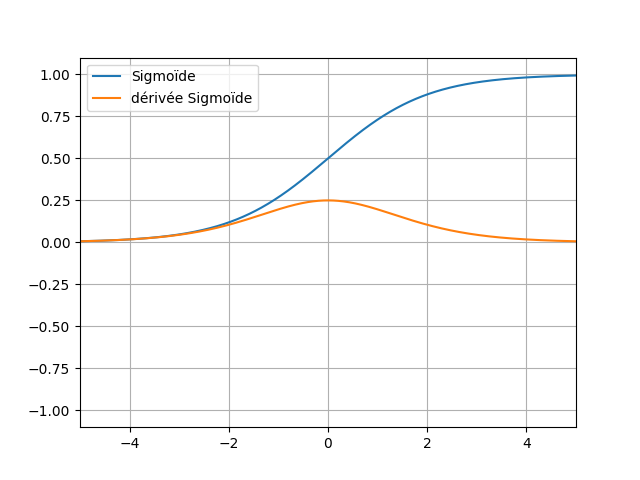
\includegraphics[width=220px]{0-Sigmoide.png}
		\caption{Sigmoïde}
	\end{figure}
\end{frame}

\begin{frame}{La fonction d'activation : TANH}
	\begin{figure}
		\centering
		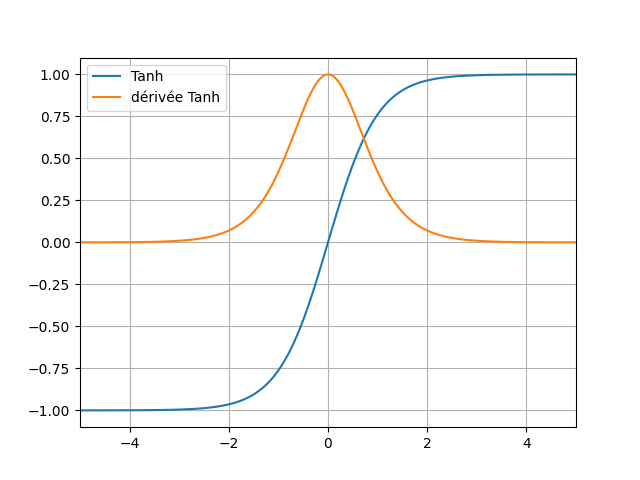
\includegraphics[width=220px]{0-Tanh.png}
		\caption{TANH}
	\end{figure}
\end{frame}

\begin{frame}{La fonction d'activation : ReLu}
	\begin{figure}
		\centering
		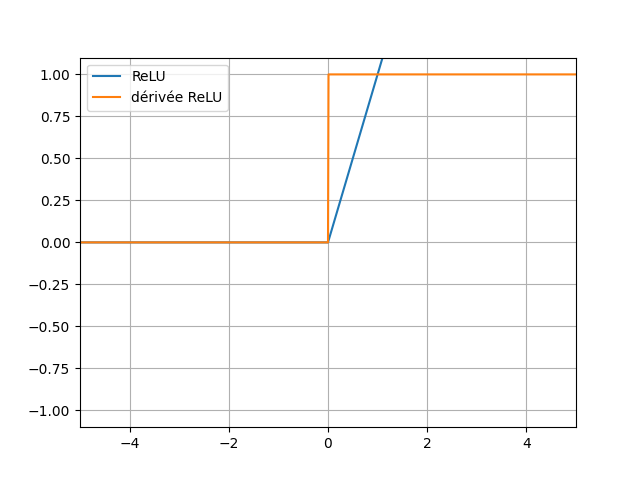
\includegraphics[width=220px]{0-ReLU.png}
		\caption{ReLu}
	\end{figure}
\end{frame}

% La rétropropagation classification
\begin{frame}{La rétropropagation pour la classification}
	\begin{block}{Cross-entropy}
		La fonction d'erreur des problèmes de classification est Cross-entropy : \\
		• $L\ \ \ = -\sum_{k=1}^{n}y_ilog(p_i)$ avec $y_i$ la sortie attendue \\
		• $\dfrac{\partial L}{\partial a_i} = p_i - y_i$
	\end{block}
\end{frame}


% Reconnaissance d'image de vêtement

\begin{frame}{Une base de données plus complexe}
    \begin{block}{Description}
        Images de taille $28 \times 28$ pixels en noir et blanc : \\
        \quad - 60 000 images pour l'entrainement. \\
        \quad - 10 000 autres pour la vérification.
    \end{block}
    \begin{columns}
        \begin{column}{0.5\textwidth}
            \begin{figure}
                \centering
                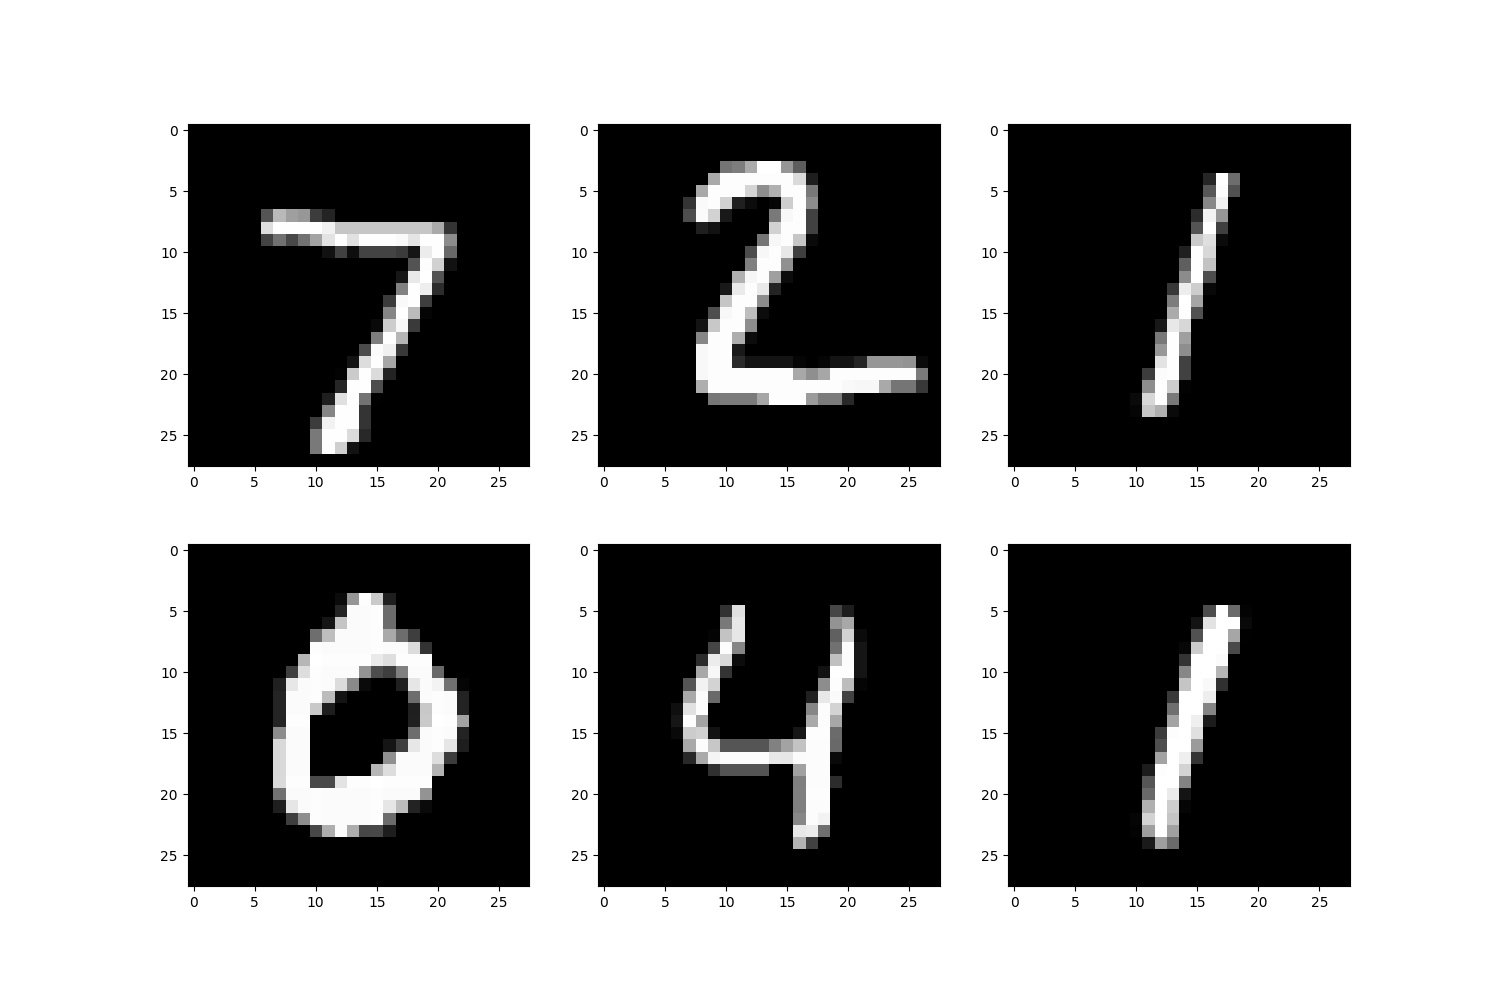
\includegraphics[width=\textwidth]{1-mnist.jpg}
                \caption{MNIST}
            \end{figure}
        \end{column}
        \begin{column}{0.5\textwidth}
            \begin{figure}
                \centering
                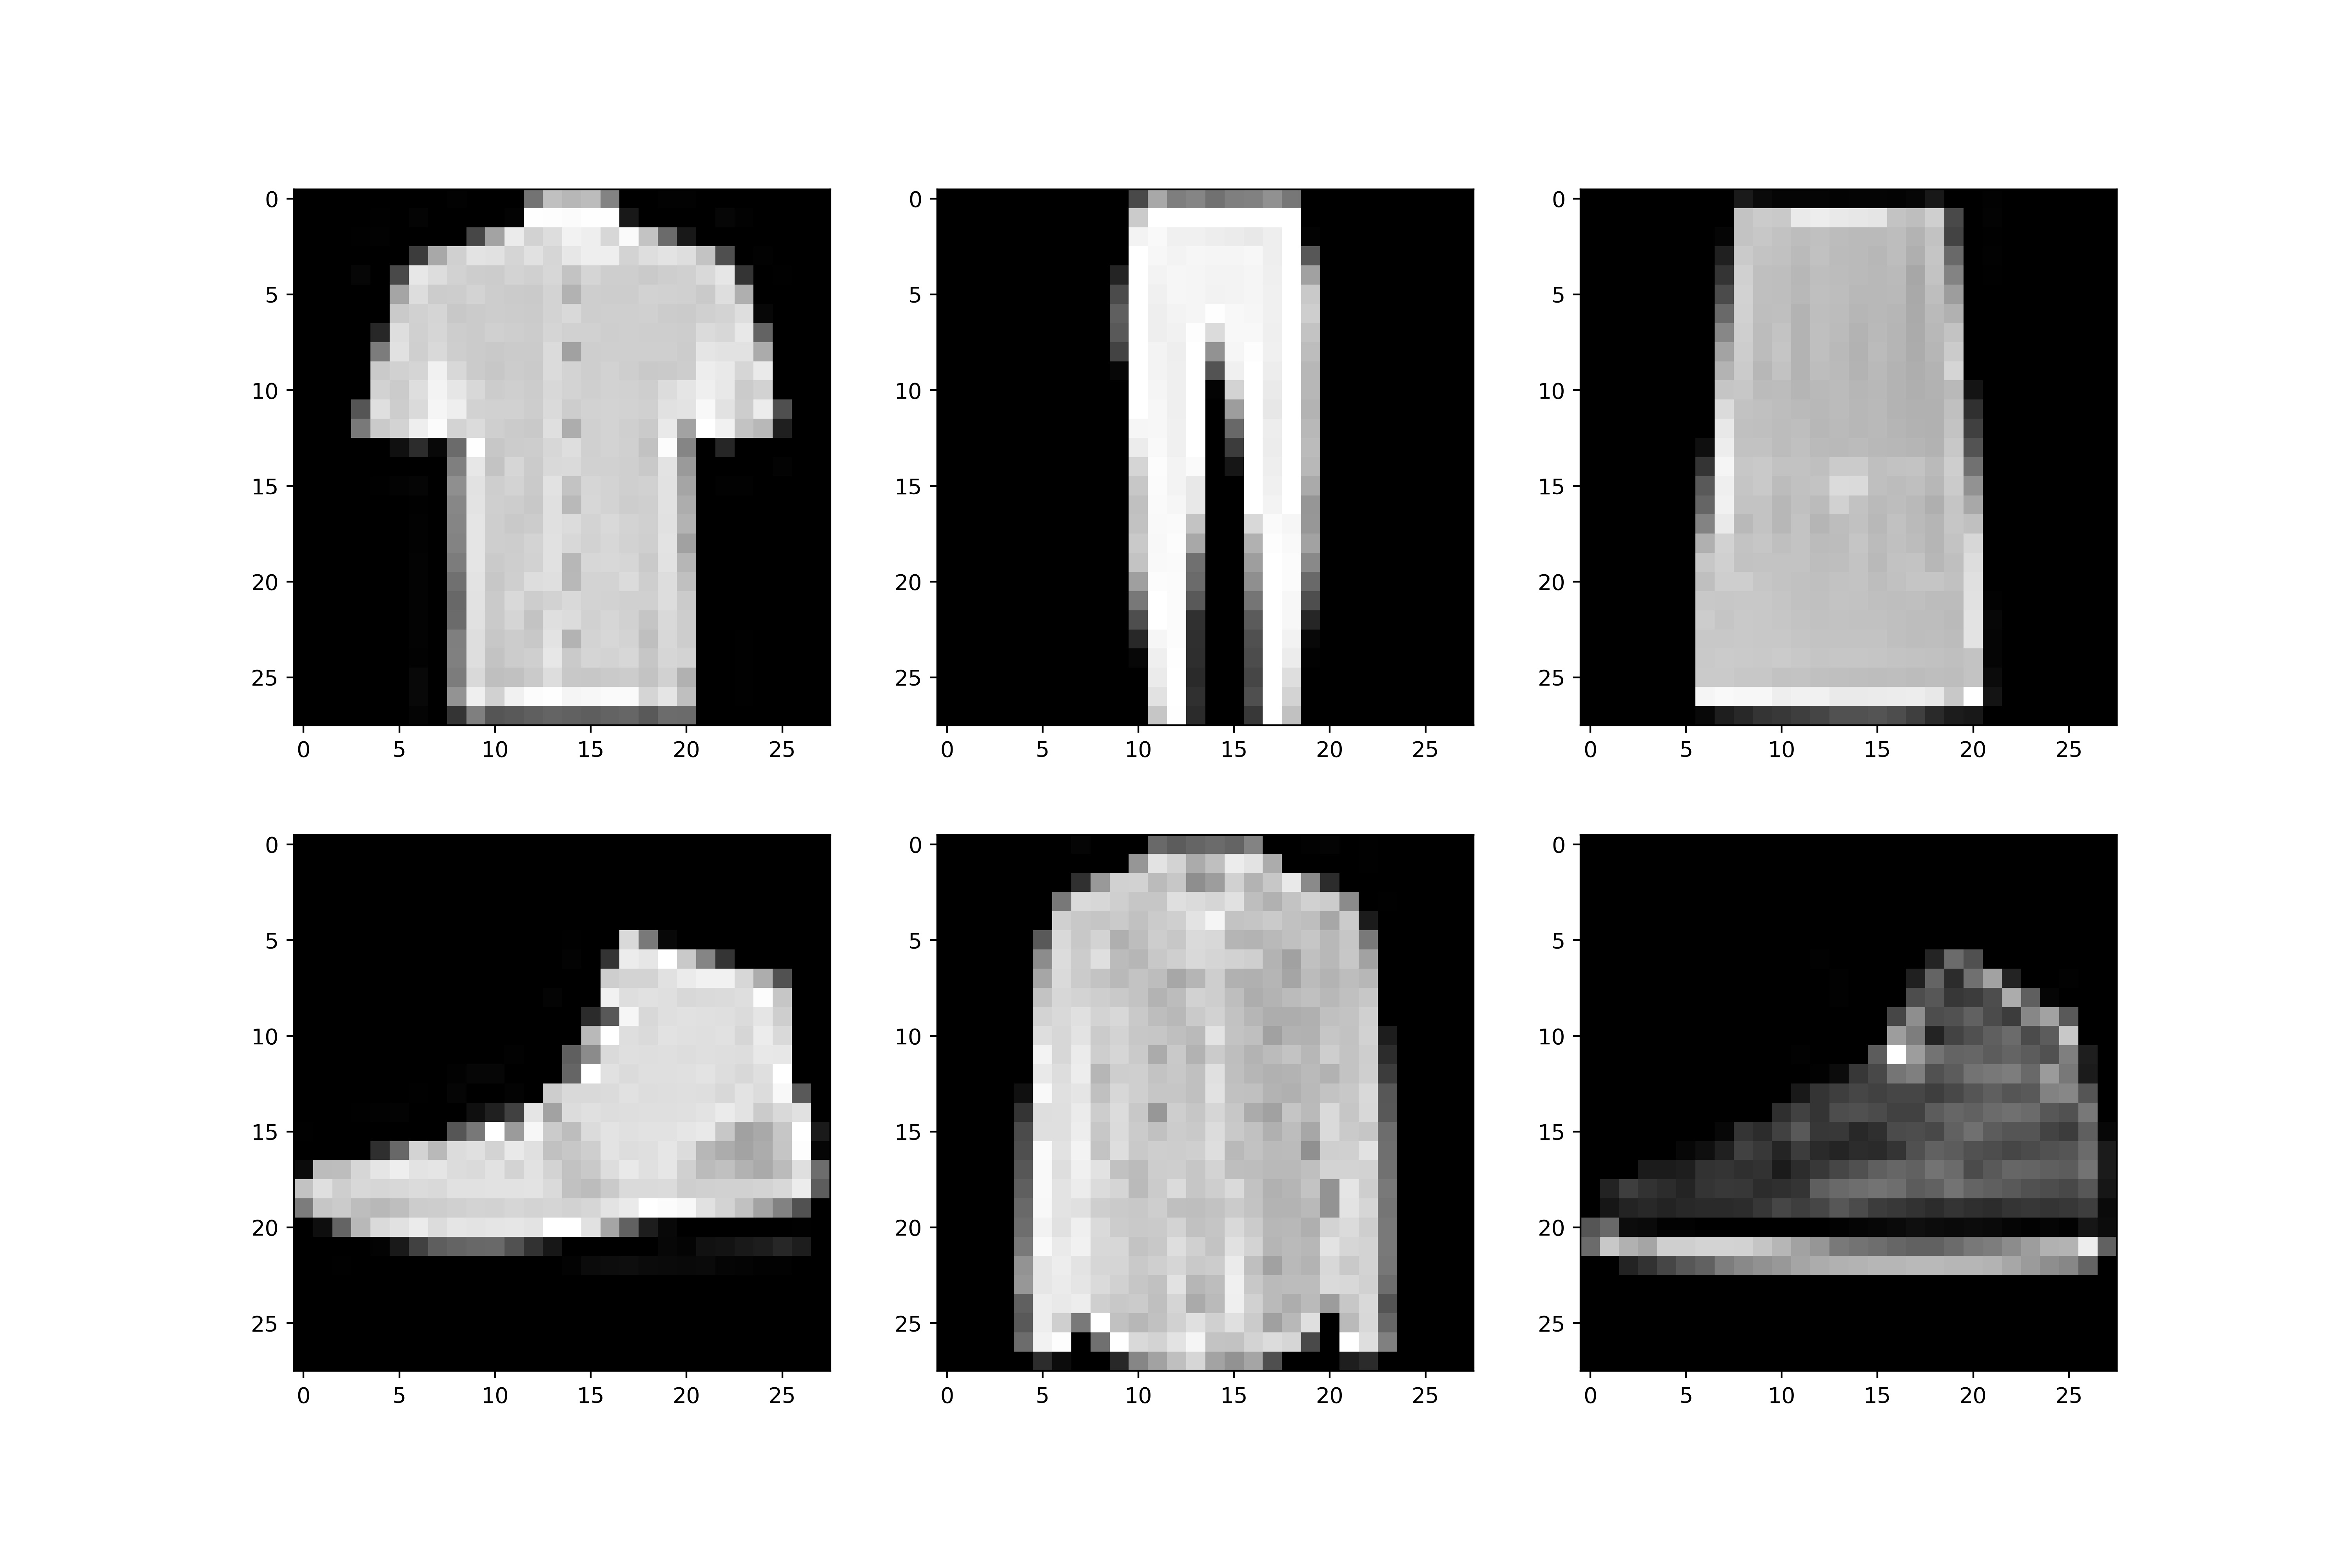
\includegraphics[width=\textwidth]{8-fashion-mnist.jpg}
                \caption{Fashion MNIST}
            \end{figure}
        \end{column}
    \end{columns}
\end{frame}


\begin{frame}{Mes résultats}
    \begin{columns}[T]
        \begin{column}{.75\textwidth}
            \begin{figure}
                \centering
                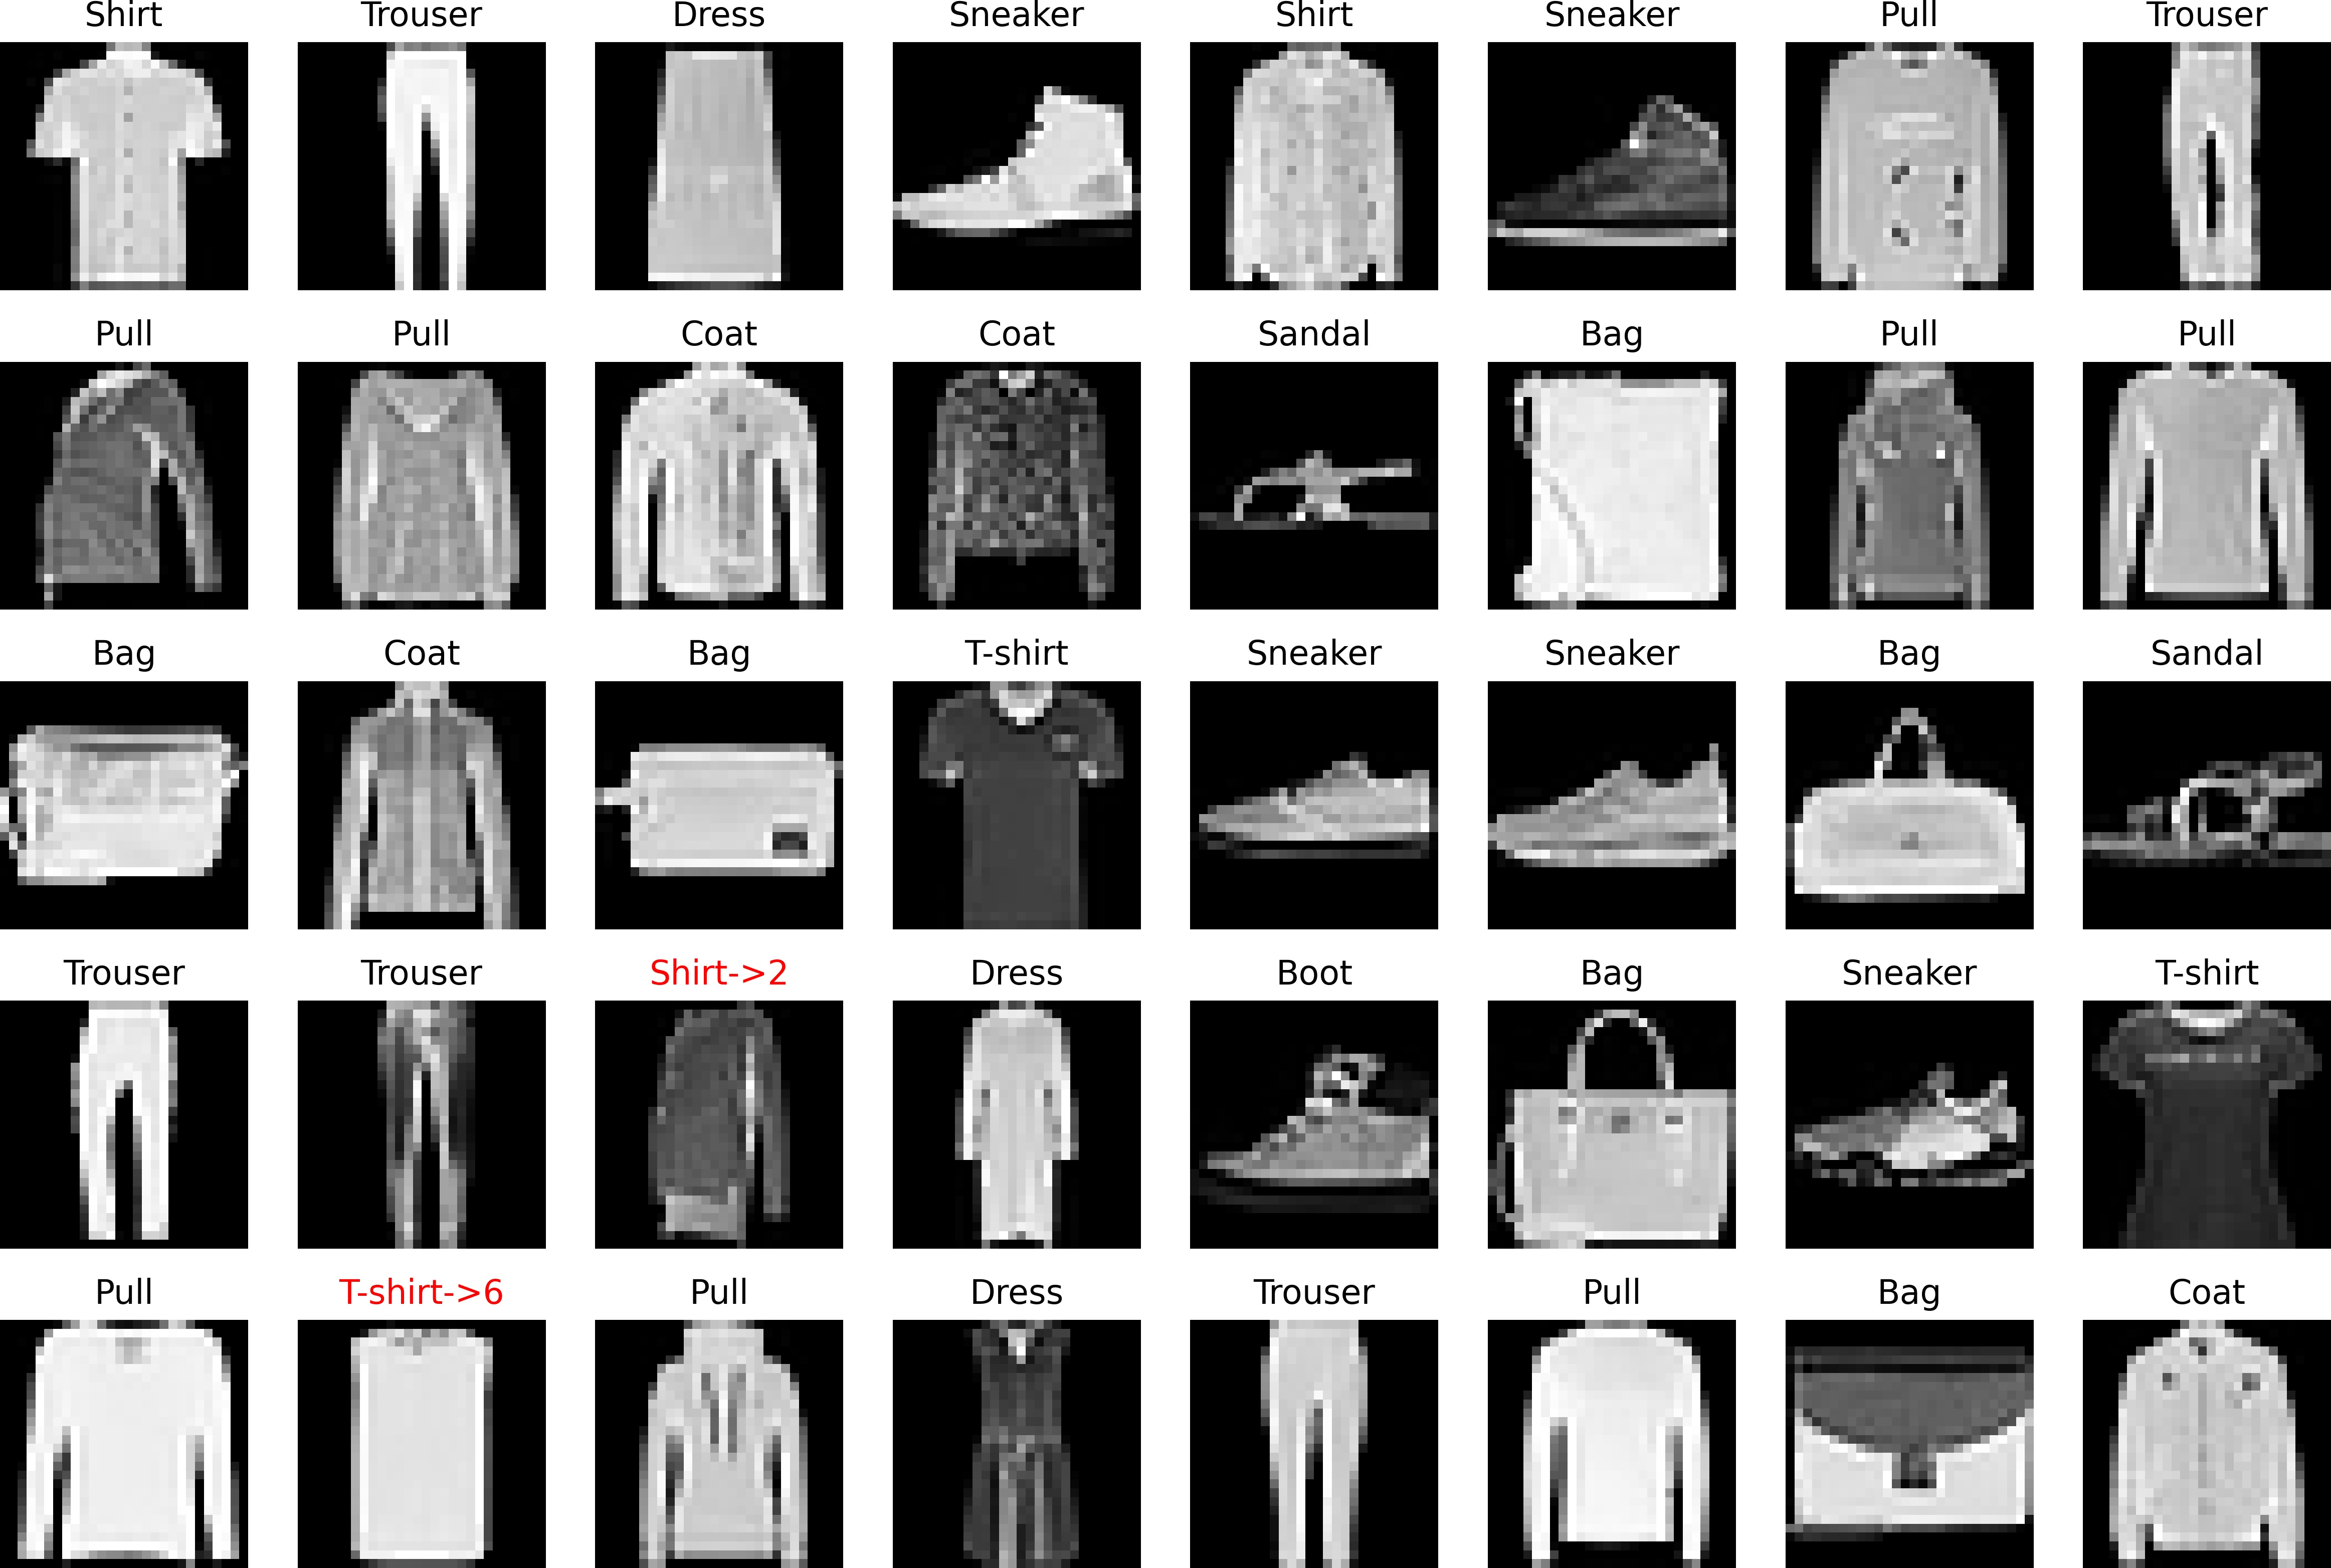
\includegraphics[width=\textwidth]{7-Resultat.jpg}
                \caption{Exemple sur un échantillon de 40 images $Fashion\ MNIST$}
            \end{figure}
        \end{column}
        \hfill
        \begin{column}{.25\textwidth}
            \bigskip	\bigskip	\bigskip
            \lstinputlisting[language=Python, firstline=15]{6-fashionDico.py}
        \end{column}
    \end{columns}
\end{frame}



% Transfert d'apprentissage
\begin{frame}[fragile, allowframebreaks]{Réseau de neurones modèle}
    \lstinputlisting[language=Python]{7-model}
\end{frame}

\begin{frame}[fragile, allowframebreaks]{Réseau de neurones adapté}
    \lstinputlisting[language=Python]{9-model2}
\end{frame}